\documentclass[conference]{IEEEtran}
\usepackage[T1]{fontenc}
\usepackage{cite,amsmath,amssymb,graphicx,booktabs,array,flushend}
\usepackage{tikz}
\usetikzlibrary{arrows.meta,positioning,calc}
\usepackage[hidelinks]{hyperref}
\hypersetup{pdftitle={Wearable Gesture Controller: Submission 2},
pdfauthor={Arya Choudhary, Sanika Singh, Vishad Sharma},
pdfsubject={ICT 3132 Embedded Systems, MIT Manipal}}
% Generated from demo/artifacts/metrics.json. Synthetic data and host timing only.
\newcommand{\TestWindows}{200}
\newcommand{\TestAccuracy}{100.0\%}
\newcommand{\MacroFone}{1.000}
\newcommand{\MacroPrecision}{1.000}
\newcommand{\MacroRecall}{1.000}
\newcommand{\AcceptedWindows}{150}
\newcommand{\BackgroundCommands}{0}
\newcommand{\MedianLatency}{0.668}
\newcommand{\PninetyfiveLatency}{0.949}
\newcommand{\WeightBytes}{4880}
\newcommand{\CheckpointBytes}{7720}

\begin{document}
\title{Wearable Gesture Controller: An IMU-Based Edge Device for Gesture-Driven Smart Home Control}
\author{\IEEEauthorblockN{Arya Choudhary, Sanika Singh, and Vishad Sharma}
\IEEEauthorblockA{School of Computer Engineering, Manipal Institute of Technology, Manipal, India\\
ICT 3132 Embedded Systems, V Semester B.Tech. (IT), Submission 2\\
Registration numbers: 240911438, 240911664, and 240911580, respectively}}
\maketitle
\begin{abstract}
Wrist-motion input could complement smart-home interfaces for people whose speech, reach, or dexterity makes conventional controls difficult to use. This project proposes an inertial measurement unit (IMU)-to-command architecture and implements a small, hardware-free software demonstration. The executable pipeline generates explicitly synthetic six-channel streams, applies causal filtering and training-only normalization, forms fixed-length windows, and classifies them with a 16-unit gated recurrent unit (GRU). A background class and confidence threshold produce a no-command outcome. Independent recordings are assigned to training, validation, and test partitions before windowing. On \TestWindows{} held-out synthetic windows, the recorded run obtained \TestAccuracy\ accuracy and macro-F1 of \MacroFone. These values show that the code learns its deliberately simple signal generator; they do not estimate real-world gesture accuracy. The report reviews ten recent research papers, identifies an application-specific integration gap, and discusses buffering, operator support, memory, latency, and optional quantization. No MCU deployment, physical appliance control, or power measurement is claimed. Scopus coverage of the reviewed papers remains unverified and requires institutional confirmation.
\end{abstract}
\begin{IEEEkeywords}
embedded systems, IMU, gesture recognition, GRU, synthetic data, edge inference, accessibility
\end{IEEEkeywords}

\section{Introduction and Problem Statement}
Smart-home interaction commonly relies on switches, touchscreens, remote controls, or voice assistants. These interfaces assume particular abilities in reach, speech, or fine motor control. A motion-based interface could provide an additional option for users who can perform comfortable, repeatable wrist movements. It would complement existing accessible controls rather than meet every user's needs. Accessibility benefit must ultimately be established with users, not inferred from classification scores.

An IMU supplies three accelerometer and three gyroscope channels without a camera's dependence on lighting or line of sight. A local classifier could translate a short motion sequence into a symbolic command without transmitting raw sensor traces to a cloud service. However, everyday movements can resemble intentional gestures. A useful interface therefore requires both recognition and a reliable no-command path, together with limits on processing delay and resource use.

The project synopsis proposes a wearable controller, an LSTM baseline, a lightweight alternative, compression, and a receiver for smart-home control. Submission 2 develops that concept into a concise design and a working laptop demonstration. The problem addressed here is: \emph{how can a bounded six-channel processing pipeline translate motion-like input into commands, reject background or uncertain predictions, and expose the evidence still needed for embedded deployment?} The implementation is restricted to a reproducible software pipeline. Wireless links and physical actuation remain proposed extensions.

The demonstration uses synthetic data because a suitable real wrist-command dataset could not be obtained and verified under the available network access. Synthetic streams make preprocessing, tensor shapes, split separation, prediction, and command mapping inspectable. They cannot establish clinical usefulness, generalization to people, or robustness to arbitrary everyday motion. All empirical results in this report refer exclusively to that synthetic software experiment.

\section{Focused Literature Survey}
The review covers ten distinct papers published in 2020--2022, within the required 2020--2026 interval. Titles, author records, publication years, venues, and publication/preprint identifiers were checked against accessible author or laboratory repositories. Publisher and Scopus endpoints were blocked by the environment's network policy. Consequently, \emph{zero papers have independently verified Scopus coverage in this package}; the faculty requirement of ten verified indexed papers is still outstanding. The accompanying source audit distinguishes publication DOIs from associated preprint DOIs and preserves verification evidence. A DOI or a familiar venue alone is not treated as proof of indexing.

\subsection{Wearable and Inertial Recognition}
Zhou \emph{et al.}'s TinyHAR combines local temporal processing, cross-channel interaction, and global temporal modelling to obtain a lightweight activity-recognition model \cite{tinyhar}. Abedin \emph{et al.} use cross-channel interaction and temporal attention to improve wearable activity representations in Attend and Discriminate \cite{attend}. These works motivate retaining both temporal and multichannel information. Their reported activity-recognition results do not establish performance for this project's command vocabulary or rejection policy.

Saha \emph{et al.}'s TinyOdom addresses inertial navigation with hardware-aware model design and quantization-aware search \cite{tinyodom}. It demonstrates the importance of sensor disturbances and target-aware resource constraints in an inertial application. Its navigation task and temporal convolutional models differ from command classification, so its resource or accuracy figures cannot be transferred to the present GRU.

\subsection{Resource-Aware Embedded Learning}
MCUNet jointly designs network architecture and an inference engine for resource-limited IoT devices \cite{mcunet}. MCUNetV2 introduces patch-based inference to address peak activation memory \cite{mcunetv2}. DORY explicitly manages tiling and data transfers when deploying neural networks on low-cost MCUs \cite{dory}. These studies show why parameter count alone is inadequate: activation lifetimes, buffers, operator implementations, and the memory hierarchy affect feasibility. Their demonstrated execution paths are not evidence that an arbitrary recurrent graph will run on every MCU.

Once-for-All specializes a trained network for deployment constraints \cite{onceforall}. TinyTL reduces activation-memory demands for on-device adaptation \cite{tinytl}, while On-Device Training Under 256KB Memory combines algorithm and runtime design for constrained training \cite{tinytraining}. These studies motivate task- and target-specific decisions, but architecture search and on-device training would add unnecessary complexity to the present student demonstration. Training is therefore performed offline on a host, and the selected GRU has a fixed, small architecture.

MLPerf Tiny treats embedded inference quality, latency, and energy as separate benchmarking dimensions \cite{mlperf}. That distinction guides the present evaluation: synthetic classification quality and host timing are reported, while MCU memory, MCU latency, and power remain unmeasured. Table~\ref{tab:literature} connects the reviewed themes to the local design gap; it does not claim an exhaustive survey or that earlier authors omitted every listed issue.

\begin{table}[t]
\caption{Literature Themes and Their Implications for This Project}
\label{tab:literature}\centering\small
\begin{tabular}{@{}>{\raggedright\arraybackslash}p{.32\columnwidth}>{\raggedright\arraybackslash}p{.61\columnwidth}@{}}
\toprule
Reviewed work & Implication and remaining local question\\
\midrule
TinyHAR; Attend and Discriminate \cite{tinyhar,attend} & Preserve time and channel structure; command rejection and user transfer need separate evidence.\\
TinyOdom \cite{tinyodom} & Inertial robustness and hardware constraints matter; navigation results do not validate gestures.\\
MCUNet; MCUNetV2; DORY \cite{mcunet,mcunetv2,dory} & Budget activations and data movement, not just weights; verify recurrent kernels.\\
Once-for-All; TinyTL; constrained training \cite{onceforall,tinytl,tinytraining} & Adapt design to target limits; keep this demonstration fixed and host-trained.\\
MLPerf Tiny \cite{mlperf} & Separate quality, latency, memory, and energy; do not substitute laptop timing for MCU measurements.\\
\bottomrule
\end{tabular}
\end{table}

\section{Research Gap, Objectives, and Contributions}
The reviewed literature supports temporal modelling, target-aware execution, and multidimensional evaluation. It does not supply evidence for this project's particular gesture-to-command pipeline. The specific gap addressed in this mini-project is an \emph{inspectable integration} of six-channel preprocessing, fixed-size windowing, a compact temporal classifier, background handling, and command rejection, with clearly separated software and hardware claims. This is an application-specific engineering gap, not a claim that wearable gesture control or compact recurrent models are new research topics.

The objectives are to: (1) implement a repeatable sensor-like input-to-command demonstration; (2) prevent recording/window leakage and select a checkpoint without using test labels; (3) expose a no-command path; and (4) document resource estimates and the additional checks required for MCU deployment. The contributions are runnable Python code with a small saved model, an explicit split and evaluation record, an embedded-oriented architecture, and a bounded account of what the results establish. No novel neural architecture or experimentally proven assistive benefit is claimed.

\section{Proposed Methodology and Architecture}
Fig.~\ref{fig:architecture} distinguishes the implemented laptop path from future physical components. The software processes six nominal channels, $\mathbf{x}_t=[a_x,a_y,a_z,\omega_x,\omega_y,\omega_z]^\mathsf{T}$. A future MCU could acquire equivalent channels using a timer or IMU data-ready interrupt and an I\textsuperscript{2}C/SPI driver, timestamping samples and detecting missed samples or sensor saturation. No such acquisition hardware has been built or selected.

\begin{figure*}[t]\centering
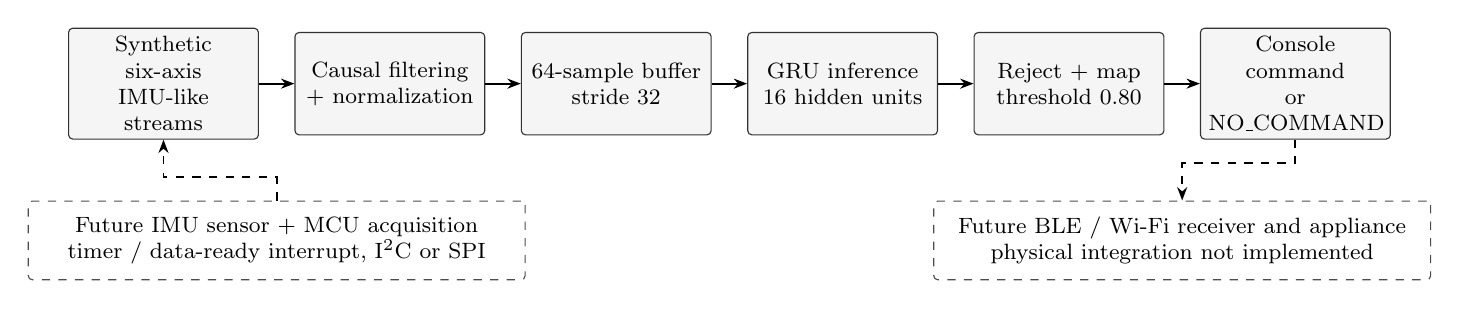
\begin{tikzpicture}[font=\footnotesize,
 box/.style={draw=black!80,fill=black!4,rounded corners=1.5pt,
 text width=22mm,align=center,minimum height=13mm,inner sep=3pt},
 future/.style={draw=black!70,dashed,text width=61mm,align=center,
 minimum height=10mm,inner sep=3pt,rounded corners=1.5pt},
 flow/.style={-{Stealth[length=1.7mm]},line width=.65pt}]
\node[box] (src) {Synthetic six-axis\\IMU-like streams};
\node[box,right=4.5mm of src] (pre) {Causal filtering\\+ normalization};
\node[box,right=4.5mm of pre] (win) {64-sample buffer\\stride 32};
\node[box,right=4.5mm of win] (model) {GRU inference\\16 hidden units};
\node[box,right=4.5mm of model] (map) {Reject + map\\threshold 0.80};
\node[box,right=4.5mm of map] (out) {Console command\\or NO\_COMMAND};
\foreach \a/\b in {src/pre,pre/win,win/model,model/map,map/out}
 \draw[flow] (\a) -- (\b);
\node[future,below=8mm of $(src.south)!0.5!(pre.south)$] (sensor)
 {Future IMU sensor + MCU acquisition\\timer / data-ready interrupt, I\textsuperscript{2}C or SPI};
\node[future,below=8mm of $(map.south)!0.5!(out.south)$] (radio)
 {Future BLE / Wi-Fi receiver and appliance\\physical integration not implemented};
\draw[flow,dashed] (sensor.north) -- ++(0,3mm) -| (src.south);
\draw[flow,dashed] (out.south) -- ++(0,-3mm) -| (radio.north);
\end{tikzpicture}

\caption{Sensor-to-command architecture. Solid blocks are exercised by the laptop software using synthetic input. Dashed components are proposed physical extensions only; no sensor, MCU, receiver, wireless link, or appliance is required to run this demonstration.}
\label{fig:architecture}
\end{figure*}

\subsection{Acquisition, Filtering, and Windowing}
The chosen software settings are a nominal $50$~Hz sample rate, $64$ samples per window, and a stride of $32$ samples. A window represents $1.28$~s of generated signal, with a new window opportunity every $0.64$~s. These are design timings, not measured response latency. A future fixed-size ring buffer would retain the most recent samples; the host demonstration forms the equivalent windows from finite arrays rather than implementing an interrupt-driven driver.

A causal first-order filter is independently reset at each recording boundary:
\begin{equation}
\mathbf{y}_0=\mathbf{x}_0,\qquad
\mathbf{y}_t=0.35\mathbf{x}_t+0.65\mathbf{y}_{t-1}.
\end{equation}
This simple filter smooths noise but adds delay and is not a substitute for sensor-side anti-alias filtering. Each channel is subsequently standardized using means and standard deviations computed from \emph{unique filtered training samples only}. These constants are frozen for validation, testing, and saved-model inference. The model input is the full $64\times6$ sequence; feature extraction is learned inside the recurrent layer. No additional handcrafted classifier or feature-selection branch is introduced.

\subsection{Compact GRU and Analytical LSTM Reference}
The implemented classifier is a single-layer, unidirectional GRU with $16$ hidden units and a linear four-class output head. A softmax converts logits to class probabilities. The classes are background, swipe left, swipe right, and wave; they map to \texttt{NO\_COMMAND}, \texttt{LIGHT\_OFF}, \texttt{LIGHT\_ON}, and \texttt{FAN\_TOGGLE}, respectively. This vocabulary is a deliberately reduced software example, not a validated human-gesture taxonomy. A hold is excluded because stillness would require an explicit interaction context.

Each window starts from a zero recurrent state and is classified from its final hidden vector. This gives bounded, independent inference calls, though overlapping windows recompute some samples. The host implementation uses PyTorch's GRU convention with separate input and recurrent bias vectors. With $d=6$, $h=16$, and $C=4$, its parameter count is
\begin{equation}
P_{\mathrm{GRU}}=3h(d+h+2)+(h+1)C.
\end{equation}
This gives $1220$ parameters. An otherwise comparable $32$-unit LSTM would have $4h(d+h+2)+(h+1)C=5252$ parameters under the same double-bias convention. This is an \emph{analytical comparison only}: no LSTM has been trained or benchmarked. The smaller GRU payload does not establish equal accuracy or a measured speedup.

\subsection{Rejection and Command Mapping}
The decision rule is
\begin{equation}
c=\begin{cases}
\mathrm{map}(k),& k\ne0,\ p_k\ge0.80,\\
\mathrm{NO\_COMMAND},&\text{otherwise},
\end{cases}
\end{equation}
where $k=\arg\max_j p_j$ and class $0$ is background. The threshold is declared before testing rather than tuned on test performance. Background samples therefore generate no command even at high confidence. Low confidence also suppresses a command, but a softmax threshold is not a guaranteed detector of unfamiliar motion. The console prints window decisions only. Temporal persistence, cooldown, acknowledgements, and secure physical actuation are future integration tasks; this program does not claim to eliminate duplicate commands in a continuous home environment.

\subsection{Resource and Quantization Constraints}
At deployment, flash must accommodate model data, inference kernels, firmware, and constants. Peak RAM includes the ring buffer, normalized input, recurrent states, scratch arena, stack, and any radio buffers. One $64\times6$ window contains $768$ bytes of 16-bit samples or $1536$ bytes of FP32 input; these are payload calculations, not total MCU RAM. The implemented FP32 model has \WeightBytes{} bytes of parameter payload, excluding host runtime and serialization overhead.

Optional 8-bit post-training quantization could map $r\approx s(q-z)$ using scale $s$ and zero point $z$, calibrated with training data only. It has not been implemented. Integer GRU gates, nonlinearities, recurrent state handling, and conversion consistency would need verification in a chosen runtime. Wider biases or states, metadata, fallback operations, and scratch storage can limit savings; quantization can also reduce accuracy. Pruning is not part of the demonstration, and introducing zeros would not by itself reduce dense storage or latency. Arduino Nano 33 BLE, ESP32, and LPC1768-based systems are examples with different MCU, memory, peripheral, and runtime constraints, not interchangeable or verified deployment targets.

\section{Software Demonstration and Pseudocode}
\subsection{Synthetic Signal Generation and Data Separation}
The generator creates independent $192$-sample recordings with six channels in nominal acceleration and angular-velocity units. Gravity is represented by an approximately constant $a_z$ offset. Background contains low-amplitude noise and drift. Left and right examples include opposite-sign stylized angular-velocity pulses with correlated acceleration; wave examples use oscillatory acceleration and angular velocity. Frequency, phase, gain, offset, and noise vary by recording. These convenient class formulas deliberately define a learnable toy problem; they are not a validated physical simulator and do not reproduce the diversity of real wrist movement.

The fixed seed is $42$. Per class, $24$ recordings are assigned to training, $8$ to validation, and $10$ to testing \emph{before filtering and windowing}. Each recording yields five windows. The resulting partitions contain $480$, $160$, and $200$ windows from $96$, $32$, and $40$ distinct recordings, respectively. Recording IDs and generator seeds are stored in a manifest. No overlapping window or recording crosses partitions. This tests separation of synthetic recordings, not transfer between real participants.

\subsection{Training and Reproduction}
Training uses FP32 CPU execution, Adam with learning rate $0.004$, batch size $64$, and categorical cross-entropy for $30$ epochs. The checkpoint with the lowest validation cross-entropy is retained. Test labels are used only after this selection. The same fixed filtering and normalization pipeline is applied to every split. Fig.~\ref{fig:workflow} summarizes the executed process; Fig.~\ref{alg:pseudocode} presents its central logic as pseudocode.

\begin{figure}[t]\centering
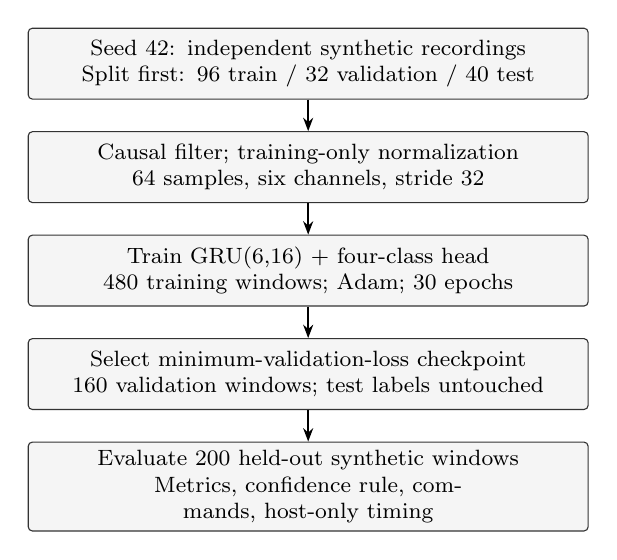
\begin{tikzpicture}[font=\footnotesize,
 box/.style={draw=black!80,fill=black!4,rounded corners=1.5pt,
 text width=69mm,align=center,minimum height=9mm,inner sep=3pt},
 flow/.style={-{Stealth[length=1.7mm]},line width=.65pt}]
\node[box] (split) {Seed 42: independent synthetic recordings\\Split first: 96 train / 32 validation / 40 test};
\node[box,below=4mm of split] (prep) {Causal filter; training-only normalization\\64 samples, six channels, stride 32};
\node[box,below=4mm of prep] (train) {Train GRU(6,16) + four-class head\\480 training windows; Adam; 30 epochs};
\node[box,below=4mm of train] (val) {Select minimum-validation-loss checkpoint\\160 validation windows; test labels untouched};
\node[box,below=4mm of val] (test) {Evaluate 200 held-out synthetic windows\\Metrics, confidence rule, commands, host-only timing};
\foreach \a/\b in {split/prep,prep/train,train/val,val/test}
 \draw[flow] (\a) -- (\b);
\end{tikzpicture}

\caption{Executed synthetic-data workflow. Split membership is assigned at recording level before windows exist. Only training data fit normalization and model weights; validation selects the checkpoint. Test data measure the final software pipeline. Quantization and MCU deployment are outside this executed path.}
\label{fig:workflow}
\end{figure}

\begin{figure}[t]
\centering
\fbox{\begin{minipage}{0.94\columnwidth}\footnotesize
\textbf{Algorithm 1: Synthetic input to command}\\[2pt]
1. Set seed $42$; assign independent recording IDs to splits.\\
2. Generate six-axis signals for each labelled recording.\\
3. Causally filter each recording; reset filter at boundaries.\\
4. Fit normalization constants from training samples only.\\
5. Normalize all splits with those frozen constants.\\
6. Form 64-sample windows, stride 32, within each recording.\\
7. Train GRU; retain lowest-validation-loss checkpoint.\\
8. For each held-out test window:\\
\hspace*{1em}$p\leftarrow\mathrm{softmax}(\mathrm{GRU}(\mathrm{window}))$.\\
\hspace*{1em}$k\leftarrow\arg\max p$.\\
\hspace*{1em}If $k$ is background or $p_k<0.80$:\\
\hspace*{2em}$c\leftarrow\mathrm{NO\_COMMAND}$.\\
\hspace*{1em}Else: $c\leftarrow\mathrm{command\_map}[k]$.\\
\hspace*{1em}Print label, confidence, and $c$.\\
9. Save metrics, split manifest, model, and example output.
\end{minipage}}
\caption{Pseudocode of the implemented demonstration.}
\label{alg:pseudocode}
\end{figure}

The supplied checkpoint allows an immediate rerun; a training flag rebuilds it. The package also records Python, NumPy, and PyTorch versions and the host environment. Seven automated checks exercise group separation, training-only normalization, causality, malformed input rejection, command rules, a known confusion matrix, and model/window dimensions. These tests check implementation properties; passing them does not validate assistive use.

\section{Results, Discussion, and Limitations}
\subsection{Actual Synthetic Software Results}
Table~\ref{tab:results} reports the saved run, not hypothetical values. Precision, recall, and F1 are computed from argmax predictions before threshold-based command rejection; macro averages include all four classes with equal class weighting. Accuracy is $\sum_k TP_k/n$, precision is $TP_k/(TP_k+FP_k)$, recall is $TP_k/(TP_k+FN_k)$, and $F1_k$ is the harmonic mean of precision and recall. A zero denominator is assigned zero in the implementation. All test classes have support $50$.

\begin{table}[t]
\caption{Recorded Synthetic Test and Host Results}
\label{tab:results}\centering\small
\begin{tabular}{@{}lr@{}}\toprule
Metric & Recorded value\\\midrule
Held-out synthetic windows & \TestWindows{} (40 recordings)\\
Accuracy & \TestAccuracy\ \\
Macro precision / recall / F1 & \MacroPrecision{} / \MacroRecall{} / \MacroFone{}\\
Accepted command windows & \AcceptedWindows{} of 150 gesture windows\\
Commands on synthetic background & \BackgroundCommands{} of 50 windows\\
Host median / p95 model latency & \MedianLatency{} / \PninetyfiveLatency{} ms\\
FP32 parameters / weight payload & 1220 / \WeightBytes{} bytes\\
Saved checkpoint size & \CheckpointBytes{} bytes\\\bottomrule
\end{tabular}
\end{table}

The confusion matrix is diagonal with $50$ correct windows per class. The first held-out examples print background $\rightarrow$ \texttt{NO\_COMMAND}, left $\rightarrow$ \texttt{LIGHT\_OFF}, right $\rightarrow$ \texttt{LIGHT\_ON}, and wave $\rightarrow$ \texttt{FAN\_TOGGLE}. Actual confidences and commands are preserved in the output transcript. All \AcceptedWindows{} accepted gesture-window commands were correct on this generated test set. A separate unit check verifies that a non-background maximum probability of $0.70$ is suppressed at the $0.80$ threshold.

Perfect toy-data scores are unsurprising because the generator creates simple, separable class patterns and train/test recordings share those formulas. They demonstrate that the pipeline can learn and map those patterns; they provide \emph{no estimate of real-world recognition accuracy}. The synthetic background test also does not establish a real false-activation rate per hour. There is no real-user dataset, external evaluation population, or physical gesture ground truth.

\subsection{Timing and Embedded Interpretation}
Model timing uses a prepared, batch-one input, CPU inference mode, one PyTorch thread, ten warm-up calls, and $100$ timed calls. The median and p95 in Table~\ref{tab:results} describe this host run and can vary on another laptop. They exclude acquisition, window filling, filtering, confidence mapping, and output transport. They are neither end-to-end response delay nor MCU latency. Host framework overhead and optimized CPU kernels prevent direct extrapolation to a microcontroller.

The weight payload is computed from actual FP32 tensors; checkpoint size additionally includes serialization and saved constants. Neither is a measurement of firmware flash or peak MCU RAM. A future target evaluation would inspect a linker map, inference-arena allocation, stack high-water marks, and concurrent buffers. Power would require a defined supply boundary and voltage/current measurement; energy would be $E=\int V(t)I(t)\,dt$. None of those hardware measurements has been performed, and battery life is not estimated.

\subsection{Limitations and Future Work}
The principal limitation is the synthetic signal distribution: real motion introduces variable placement, orientation, tremor, fatigue, incomplete gestures, and incidental activities absent here. Background is not representative of the open set of everyday movements, and confidence is not calibrated as a probability of safe action. Before physical control, the design would need real labelled recordings, participant/session-separated evaluation, continuous-stream event matching, false activations per hour, duplicate suppression, and user-centred accessibility assessment.

The LSTM comparison, quantization, target selection, wireless receiver, and appliance interface remain analytical or future work. Literature indexing verification and an institution-approved similarity report are separate outstanding submission checks. Future development should first validate a suitable real-data protocol and MCU/runtime operator support, then measure on-target resource use. Additional applications or dashboards are unnecessary for the present scope.

\section{Conclusion}
Submission 2 delivers an executable six-channel synthetic processing and command-generation demonstration alongside an embedded-oriented design. A compact GRU, training-only normalization, recording-level split, background class, and confidence rejection provide a clear and reproducible software example. Actual synthetic metrics and host timings are reported with explicit boundaries; no result is presented as a real-user or MCU benchmark. The literature supports attention to temporal structure, memory behaviour, and evaluation scope while leaving indexing confirmation outstanding. The package advances the synopsis from a theoretical architecture to a working software pipeline without claiming hardware deployment or validated assistive performance.

\bibliographystyle{IEEEtran}
\bibliography{references}
\end{document}
